%%%%%%%%%%%%%%%%%%%%%%%%%%%%%%%%%%%%%%%%%%%%%%%%%%%%%%%%%%%%%%%%%%%%%%%%%%%%%%%%%%%%%%%%%%%%
%                          Procedimientos simulaciones radiación                           % 
%%%%%%%%%%%%%%%%%%%%%%%%%%%%%%%%%%%%%%%%%%%%%%%%%%%%%%%%%%%%%%%%%%%%%%%%%%%%%%%%%%%%%%%%%%%%
\chapter[Procedimientos simulaciones radiación]{Procedimientos seguidos para la realización de las simulaciones de radiación de campo cercano}\label{ch:procedimientosSimRad}

En este apéndice se detallan los pasos genéricos seguidos para la realización de las simulaciones de radiación de campo cercano y la obtención de los resultados de las potencias integradas en un respectivo rango espectral utilizando la aplicación \textbf{calculadora de campo cercano}, descrita en la sección \ref{sec:calc_campo_cercano}.

\section{Procedimientos genéricos}
Existen solo cuatro posibles casos de simulaciones de transmisión de calor por radiación de campo cercano utilizando la aplicación, estos casos son los siguientes:
\begin{itemize}
	\item Una distancia de separación y un par de materiales, uno para el emisor y otro para el receptor.
	\item Rango de distancias de separación y un par de materiales.
	\item Una distancia de separación y varias combinaciones de materiales.
	\item Rango de distancias de separación y varias combinaciones de materiales.
\end{itemize}
Los procedimientos para la realización de las simulaciones de transmisión de calor por radiación de campo cercano siguen el mismo orden de ejecución genérico. Estos procedimientos son:
\begin{itemize}
	\item Selección de la temperatura del emisor, que para este trabajo se mantiene a 1073K (800\textdegree C).
	\item Selección de las combinaciones de materiales a simular.
	\item Selección del rango de distancias a simular.
	\item Hacer clic sobre el botón \textbf{Calculate}.
\end{itemize}
%%%%%%%%%%%%%%%%%%%%%%%%%%%%%%%%%%%%%%%%%%%%%%%%%%%%%%%%%%
%        Distancia fija y un par de materiales           %
%%%%%%%%%%%%%%%%%%%%%%%%%%%%%%%%%%%%%%%%%%%%%%%%%%%%%%%%%%
\section{Distancia fija y un par de materiales} \label{DfMf}
Este caso consiste en una sola distancia de separación, un material para el emisor y otro material para el receptor.
Para proceder con la simulación se siguen los siguientes pasos:
\begin{enumerate}
	\item Seleccionar el material de la placa superior en \textbf{Superior plate} (figura \ref{unParMat}). 
	\item Seleccionar el material de la placa inferior en \textbf{Inferior plate}.
	\item Seleccionar la distancia (figura \ref{unaDistancia}). 
%%%%%
		\begin{figure}[H]
			\centering
			\begin{subfigure}[b]{.48\textwidth}
				\centering
					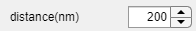
\includegraphics{figuras/unaDistancia.PNG}
				\caption{ }
				\label{unaDistancia}
			\end{subfigure} \hfill
			\begin{subfigure}[b]{.48\textwidth}
				\centering
					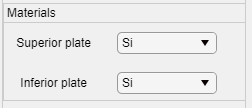
\includegraphics{figuras/unParMat.PNG}
					\caption{ }
				\label{unParMat}
			\end{subfigure}
			\caption{Seleccionador de una distancia de separación en nanometros (\subref{unaDistancia}) y seleccionar de los materiales de emisor (Superior plate) y receptor (Inferior plate) (\subref{unParMat}) de la calculadora de campo cercano.}
			\label{fig:sencillo}
		\end{figure}	
%%%
	\item Hacer click sobre el botón \textbf{Calculate}.
	\item Esperar que el indicador de estado pase de \textit{Running...}, color rojo del indicador (figura \ref{fig:indicador_Running2}), a \textit{StdBy}, color verde del indicador (figura \ref{fig:indicador_StdBy2}), es decir, esperar que termine la simulación.
\end{enumerate}
		%% figuras de estados
	\begin{figure}[H]
		\centering
		%% Figura 1
		\begin{subfigure}[b]{0.3\textwidth}
			\centering
			
\includegraphics[width=\textwidth]{figuras/Procedimiento_Simulaciones/Radiacion/estado_changed}%
			\caption{Changed}%
			\label{fig:indicador_Changed2}%
		\end{subfigure}
		\hfill
		%% Figura 2
		\begin{subfigure}[b]{0.3\textwidth}
			\centering
			
\includegraphics[width=\textwidth]{figuras/Procedimiento_Simulaciones/Radiacion/estado_running}%
			\caption{Running}%
			\label{fig:indicador_Running2}%
		\end{subfigure}
		\hfill
		%% Figura 3
		\begin{subfigure}[b]{0.3\textwidth}
			\centering
			
\includegraphics[width=0.9\textwidth]{figuras/Procedimiento_Simulaciones/Radiacion/estado_stdby}%
			\caption{StdBy}%
			\label{fig:indicador_StdBy2}%
		\end{subfigure}
		\hfill
		\caption{Indicadores del estado actual del sistema. (\subref{fig:indicador_Changed2}) Indicador del estado \textbf{Changed} o estado de cambio, se activa cuando se produce algún cambio en los datos seleccionados para simular. (\subref{fig:indicador_Running2}) Indicador del estado \textbf{Running} o corriendo, se activa cuando estando en el estado \textbf{Changed} se hace clic al botón \textbf{Calculate} y corre la simulación. (\subref{fig:indicador_StdBy2}) Indicador del estado \textbf{StdBy}, se activa cuando termina la simulación, avisando que está a la espera de algún cambio.}
		\label{fig:indicadorLED2}
	\end{figure}
	%%%%%%%%%%%%%%%%%%%%%%%%%%%%%%%%%%%%%%%%%%%%%%%%%%%%%%%%%%%%%
	%       Rango de distancias y un par de materiales         %
%%%%%%%%%%%%%%%%%%%%%%%%%%%%%%%%%%%%%%%%%%%%%%%%%%%%%%%%%%%%%%%
\section{Rango de distancias y un par de materiales}\label{DrMf}
Este caso de simulación consiste en un rango de distancias de separación de 100 nm de paso y la combinación de un material del emisor con otro material del receptor.
Para proceder con la simulación se siguen los siguientes pasos:
	\begin{enumerate}
		\item Seleccionar el material de la placa superior en \textbf{Superior plate} (figura \ref{unParMat}).
		\item Seleccionar el material de la placa inferior en \textbf{Inferior plate}.
		\item Hacer click sobre el checkbox \textbf{Distance Range} (figura \ref{fig:check_distances2}).
		\item Hacer click sobre el botón \textbf{set} del \textbf{Distance Range}, que produce que aparezca la ventana de la figura \ref{fig:set_distances2}.
		\item Seleccionar el rango de distancias deseado o el checkbox \textbf{Full Range}, según lo que se desee. Para este trabajo se selecciona el checkbox \textbf{Full Range}.
		\item Hacer click en \textbf{Accept} de la nueva ventana.
		\item Hacer click sobre el botón \textbf{Calculate} y esperar a que termine de ejecutarse la simulación.
	\end{enumerate}
	%%%%%%     FIGURAS   
		\begin{figure}[H]%
		\begin{subfigure}[b]{0.48\textwidth}
			\centering
				
\includegraphics[width=0.6\textwidth]{figuras/Procedimiento_Simulaciones/Radiacion/check_distances2.png}
			\caption{Checkbox de distancias}
			\label{fig:check_distances2}
		\end{subfigure}
		\hfill
		\begin{subfigure}[b]{0.48\textwidth}
			\centering
				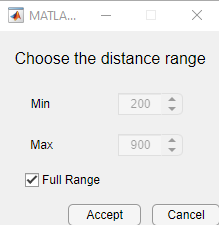
\includegraphics[width=0.6\textwidth]{figuras/Procedimiento_Simulaciones/Radiacion/set_distances_fullrange.png}
			\caption{Set de distancias}
			\label{fig:set_distances2}
		\end{subfigure}
		\caption{(\subref{fig:check_distances2}) Casilla para la selección de la opción de simular un rango de distancias. (\subref{fig:set_distances2}) Ventana para la selección del rango de distancias a simular.}%
		\label{fig:checkboxes2}%
		\end{figure}
	%%%%%%%%%%%%%%%%%%%%%%%%%%%%%%%%%%%%%%%%%%%%%%%%%%%
	%        Distancia fija y varios materiales       %
	%%%%%%%%%%%%%%%%%%%%%%%%%%%%%%%%%%%%%%%%%%%%%%%%%%%
	\section{Distancia fija y varios materiales}\label{DfMr}
Este caso de simulación consiste en una sola distancia de separación y varias combinaciones de los materiales del emisor con los del receptor. Para proceder con la simulación se siguen los siguientes pasos:
	\begin{enumerate}
			\item Hacer click sobre el checkbox \textbf{Materials Range} (figura \ref{fig:check_materials2}).
			\item Hacer click sobre el botón \textbf{set} del \textbf{Materials Range}, que produce que aparezca la ventana de la figura \ref{fig:set_materials2}.
			\item Seleccionar los materiales para la cara superior (UpFace) (figura \ref{fig:set_materials2}).
			\item Seleccionar los materiales para la cara inferior (DownFace).
			\item Hacer clic en \textbf{Accept} de la ventana emergente.
			\item Seleccionar la distancia (figura \ref{unaDistancia}). 
			\item Hacer click sobre el botón \textbf{Calculate} y esperar a que termine de ejecutarse la simulación.
	\end{enumerate}			
	%%%%%%%%%%%%%%%%%   FIGURAS  
	\begin{figure}[H]%
		\begin{subfigure}[b]{0.48\textwidth}
			\centering
				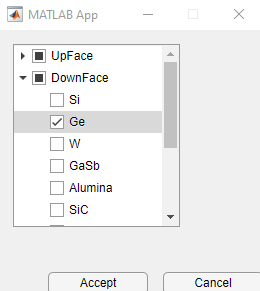
\includegraphics[width=0.6\textwidth]{figuras/Procedimiento_Simulaciones/Radiacion/set_materilas2.png}
			\caption{Set de materiales}
			\label{fig:set_materials2}
		\end{subfigure}\hfill
			\begin{subfigure}[b]{0.48\textwidth}
			\centering
				
\includegraphics[width=0.6\textwidth]{figuras/Procedimiento_Simulaciones/Radiacion/check_materials2.png}
			\caption{Checkbox de materiales}
			\label{fig:check_materials2}
		\end{subfigure}
		\caption{(\subref{fig:set_materials2}) Ventana para la selección de las combinaciones de materiales a simula, siendo \textbf{UpFace} el emisor y \textbf{DownFace} la célula.	(\subref{fig:check_materials2}) Casilla para la selección de la opción de simular una combinación de materiales.}%
		\label{fig:sets2}%
	\end{figure}	
	%%%%%%%%%%%%%%%%%%%%%%%%%%%%%%%%%%%%%%%%%%%%%%%%%%%%
	%      Rango de materiales y varios materiales     %
	%%%%%%%%%%%%%%%%%%%%%%%%%%%%%%%%%%%%%%%%%%%%%%%%%%%%
\section{Rango de materiales y varios materiales}\label{DrMr}
Este caso de simulación consiste en un rango de distancias de separación de 100 nm de paso y varias combinaciones de materiales del emisor con los del receptor. Para proceder con la simulación se siguen los siguientes pasos:
\begin{enumerate}
			\item Hacer click sobre el checkbox \textbf{Materials Range} (figura \ref{fig:check_materials2}).
			\item Hacer click sobre el checkbox \textbf{Distance Range} (figura \ref{fig:check_distances2}).
			%% MATERIALS
			\item Hacer click sobre el botón \textbf{set} del \textbf{Materials Range}, que produce que aparezca la ventana de la figura \ref{fig:set_materials2}.
			\item Seleccionar los materiales para la cara superior (UpFace) (figura \ref{fig:set_materials2}).
			\item Seleccionar los materiales para la cara inferior (DownFace).
			\item Hacer clic en \textbf{Accept} de la ventana emergente.
			%%%% DISTANCE
			\item Hacer click sobre el botón \textbf{set} del \textbf{Distance Range}, que produce que aparezca la ventana de la figura \ref{fig:set_distances2}.
			\item Seleccionar el rango de distancias deseado o el checkbox \textbf{Full Range}, según lo que se desee. Para este trabajo se selecciona el checkbox \textbf{Full Range}.
			\item Hacer click en \textbf{Accept} de la nueva ventana.
			\item Hacer click sobre el botón \textbf{Calculate} y esperar a que termine de ejecutarse la simulación.
\end{enumerate}
%%%%%%%%%%%%%%%%%%%%%%%%%%%%%%%%%%%%%%%%%%%%%%%%%%%%%%%%%%%%%%%
%     Integración de la potencia en un rango espectral        %
%%%%%%%%%%%%%%%%%%%%%%%%%%%%%%%%%%%%%%%%%%%%%%%%%%%%%%%%%%%%%%%
\section{Integraci\'{o}n de la potencia en un rango espectral}
Para proceder a la integración de las potencias obtenidas de las simulaciones, se siguen los siguientes pasos:
	%% Se acaba la figura
	\begin{enumerate}
	\item Ir a la pestaña de \textbf{Potencia}.
	\item Introducir el rango de longitudes de onda para calcular la potencia por unidad de área, siendo elegido desde el mínimo hasta 1.8 $\mu m$ que es el rango de longitudes de onda que absorbe la célula de Ge (figura \ref{fig:graficar_ejemplo2}).
	\item Hacer clic en el botón \textbf{Graph} para calcular y graficar las potencias (figura \ref{fig:graficar_ejemplo2}).
\end{enumerate}
%% Graficas de la pestaña de potencia
\begin{figure}[H]
	\centering
	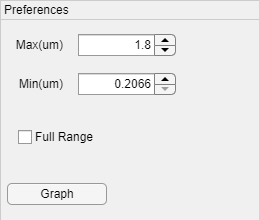
\includegraphics[width=0.30\textwidth]{figuras/Procedimiento_Simulaciones/Radiacion/graficar_ejemplo2.png}
	\caption{Preferencias para el cálculo de la potencia}
	\label{fig:graficar_ejemplo2}
\end{figure}
%%%%%%%%%%%%%%%%%%%%%%%%%%%%%%%%%%%%%%%%%
%        Guardado de los datos          %
%%%%%%%%%%%%%%%%%%%%%%%%%%%%%%%%%%%%%%%%%
\section{Guardado de los datos}
Para la extracción o guardado de los resultados obtenidos de las simulaciones, es decir, las potencias de transmisión de calor por radiación. Para guardar todos los datos disponibles de la última simulación ejecutada, las potencias frente a la longitud de onda y las potencias integradas en un rango espectral, se hace clic sobre el botón de \textbf{guardar todos}, que se observa en la figura \ref{fig:SaveAllicon}.
\begin{figure}[H]
	\centering
	\begin{subfigure}[b]{0.48\textwidth}
		\centering
		
\includegraphics[width=0.4\textwidth]{figuras/Procedimiento_Simulaciones/Radiacion/SaveButton_Cut.jpg}
		\caption{Botón de guardar actual}
		\label{fig:SaveButton_Cut}
	\end{subfigure}
  \hfill
	\begin{subfigure}[b]{0.48\textwidth}
		\centering
			
\includegraphics[width=0.40\textwidth]{figuras/Procedimiento_Simulaciones/Radiacion/SaveAllicon.jpg}
		\caption{Botón de guardar todos los resultados}
		\label{fig:SaveAllicon}
	\end{subfigure}
	\caption{(\subref{fig:SaveButton_Cut}) Botón de guardar los resultados obtenidos de los cálculos o la simulación, dependiendo de la pestaña que se encuentre el usuario de la calculadora de campo cercano. (\subref{fig:SaveAllicon}) Botón de guardar todos los resultados obtenidos de los cálculos y simulación.}
	\label{fig:saveButtons}
\end{figure}
Para guardar exclusivamente las potencias frente a la longitud de onda, se procede  air a dicha pestaña y hacer clic sobre el botón de \textbf{guardar}, que se observa en la figura \ref{fig:SaveButton_Cut}. Y para guardar exclusivamente las potencias integradas en un rango espectral, se hace clic sobre el mismo botón \textbf{guardar}.


%%%%%%%%%%%%%%%%%%%%%%%%%%%%%%%%%%%%%%%%%%%%%%%%%%%%%%%%%%%%%%%%%%%%%%%%%%%%%%%%%%%%%%%%%%%%
%                          Procedimientos simulaciones radiación                           % 
%%%%%%%%%%%%%%%%%%%%%%%%%%%%%%%%%%%%%%%%%%%%%%%%%%%%%%%%%%%%%%%%%%%%%%%%%%%%%%%%%%%%%%%%%%%%
\chapter[Procedimiento del modelado 3D]{Procedimiento para la realización del modelado 3D}\label{ch:procedimientosModelado3D}
Para la realización del modelado 3D del sistema a simular en CFD y de sus componentes se sigue el siguiente procedimiento, detallado paso a paso.
\begin{enumerate}
	\item Crear las bases cuadradas con la longitud de lado respectiva, 10m para emisor o célula y 3cm para el nano-espaciador en la escala del modelo 3D en Inventor. 
	\item Extrudir el prisma la longitud correspondiente, 2m para el emisor/célula y $h_0$ para el nano-espaciador, siendo $h$ un valor inicial cualquier en el rango de 1mm a 10mm.
	\item Crear un ensamblaje de emisor-espaciador-célula, estando la base del nano-espaciador en el centro de las bases de los otros dos componentes (figura \ref{fig:modelado3D}).
	%% PASOS PARA EL ENSAMBLAJE
	\begin{enumerate}
		\item Agregar el nano-espaciador y los dos prismas de 10m de lado.
		\item Renombrar los prismas de 10m de lado, una siendo emisor y la otra célula, para así diferenciarlas.
		\item Obtener el centro de la cara superior de la célula, mediante un dibujo con dos rectas secantes que van de una esquina a otra (figura \ref{fig:modelado3D_centro_cerca}).
		\item Aplicar una restricción con la opción \textbf{Mate} de separación nula entre la cara inferior del nano-espaciador con el centro de la cara superior de la célula,es decir, las caras entran en contacto si la distancia de separación es nula (figura \ref{fig:modelado3D_centro_cerca}).
		\item Aplicar una restricción \textbf{Mate} de separación nula entre la cara inferior del emisor y la cara superior del nano-espaciador.
		\item Aplicar una restricción \textbf{Flush} de separación nula a una cara lateral del emisor y una cara lateral de la célula.
		\item Repetir el paso anterior para las caras conjuntas, siendo el resultado final el de la figura \ref{fig:modelado3D_lejos}.
	\end{enumerate}
\begin{figure}[H]
	\centering
	\begin{subfigure}[b]{0.3\textwidth}
		\centering
			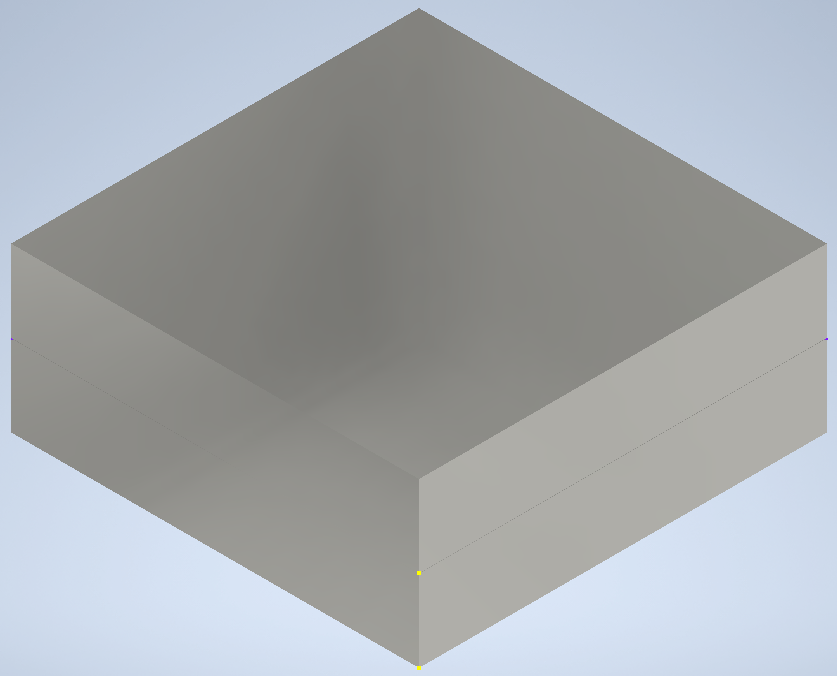
\includegraphics[width=1.00\textwidth]{figuras/Procedimiento_Simulaciones/Conduccion/modelado3D_lejos.png}
		\caption{Vista global TPV}
		\label{fig:modelado3D_lejos}
	\end{subfigure}
	\hfill
	\begin{subfigure}[b]{0.3\textwidth}
		\centering
			
\includegraphics[width=1.00\textwidth]{figuras/Procedimiento_Simulaciones/Conduccion/modelado3D_cerca.png}
		\caption{Vista cerca TPV}
		\label{fig:modelado3D_cerca}
	\end{subfigure}
	\hfill
	\begin{subfigure}[b]{0.3\textwidth}
		\centering
			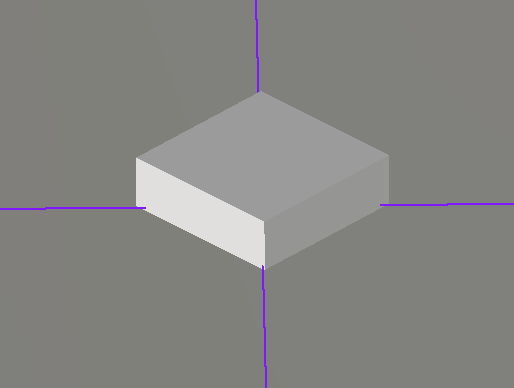
\includegraphics[width=1.00\textwidth]{figuras/Procedimiento_Simulaciones/Conduccion/modelado3D_centro_cerca.png}
		\caption{Vista cerca nano-espaciador}
		\label{fig:modelado3D_centro_cerca}
	\end{subfigure}
	\caption{Vistas del sistema TPV. (\subref{fig:modelado3D_lejos}) Vista de lejos del sistema completo de la TPV. (\subref{fig:modelado3D_cerca}) Vista del sistema TPV de cerca desde un borde. (\subref{fig:modelado3D_centro_cerca}) Vista del nano-espaciador colocado sobre el centro de una cara de la célula.}
	\label{fig:modelado3D}
\end{figure}
	\item Guardar el ensamblaje.
	\item Usar el \textbf{Active Model Assessment Tool}, que se encuentra en la pestaña de simulaciones, para generar el modelo o estudio de simulación de CFD\label{itm:pasoIniIterativo_Modelado3D}.
	\item Al abrirse CFD hacer clic en \textit{Transfer to Set Up}, dar un nombre y lanzar.
	\item Guardar el modelo o estudio de CFD \label{itm:pasoFin_Modelado3D}.
	\item Ir al ensamblaje en Inventor.
	\item Hacer clic derecho sobre el ícono del objeto correspondiente al nano-espaciador en el panel \textbf{model} y hacer clic en editar.
	\item Hacer clic derecho sobre la extrusión y seleccionar la opción de editar característica (\textbf{Edit Feature}).
	\item Modificar la altura del nano-espaciador y al terminar hacer clic en \textbf{Return} \label{itm:pasoFinIterativo_Modelado3D}.
	\item Repetir desde el paso \ref{itm:pasoIniIterativo_Modelado3D} al \ref{itm:pasoFinIterativo_Modelado3D}, excepto en la última iteración que es hasta el paso \ref{itm:pasoFin_Modelado3D}, incluido.
\end{enumerate} 
%%%%%%%%%%%%%%%%%%%%%%%%%%%%%%%%%%%%%%%%%%%%%%%%%%%%%%%%%%%%%%%%%%%%%%%%%%%%%%%%%%%%%%%%%%%%
%                          Procedimientos simulaciones radiación                           % 
%%%%%%%%%%%%%%%%%%%%%%%%%%%%%%%%%%%%%%%%%%%%%%%%%%%%%%%%%%%%%%%%%%%%%%%%%%%%%%%%%%%%%%%%%%%%
\chapter[Procedimiento simulación conducci\'{o}n]{Procedimiento para la realización de las simulaciones de CFD}\label{ch:procedimientosSimCond}
%%%  PROCEDIMIENTO CFD
Para la realización de las simulaciones de transmisión de calor por conducción en CFD se sigue el siguiente procedimiento, que se encuentra detallado paso a paso.
\begin{enumerate}
	\item Abrir el modelo o estudio correspondiente de simulación en CFD.
	\item Seleccionar el emisor y cambiar el material por defecto por el que se va a simular a escala.
	\item Seleccionar el entorno del material del emisor como variable.
	\item Seleccionar la célula y cambiar el material por defecto por el que se va a simular a escala.
	\item Seleccionar el entorno del material de la célula como variable.
	\item Hacer zoom sobre el nano-espaciador, seleccionarlo y cambiar el material por defecto por el $SiO_2$ a escala.
	\item Seleccionar el entorno del material del nano-espaciador como variable.
	\item \textbf{En el caso que la resistencia de contacto no sea nula:}
	\begin{enumerate}
		\item Esconder el emisor.
		\item Seleccionar el selector de superficies.
		\item Seleccionar la superficie superior del nano-espaciador, es decir, la superficie que hace contacto con el emisor.
		\item Cambiar el material por defecto por la resistencia de contacto a escala.
		\item Seleccionar el selector de volúmenes.
		\item Mostrar el emisor.
	\end{enumerate}
	%% PANEL DE HERRAMIENTAS
	\begin{figure}[h]
	\centering
	\begin{subfigure}[b]{0.48\textwidth}
		\centering
			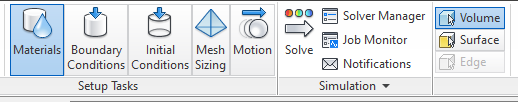
\includegraphics[width=0.9\textwidth]{figuras/Procedimiento_Simulaciones/Conduccion/paneles.png}
		\caption{Panel principal}
		\label{fig:paneles}
		\end{subfigure}
		\hfill
		\begin{subfigure}[b]{0.48\textwidth}
			\centering
			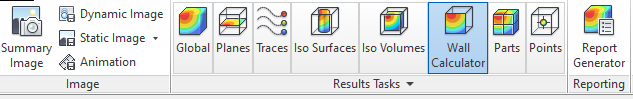
\includegraphics[width=0.9\textwidth]{figuras/Procedimiento_Simulaciones/Conduccion/paneles_resultados.png}
			\caption{Panel de resultados}
			\label{fig:paneles_resultados}
		\end{subfigure}
		\caption{(\subref{fig:paneles}) Panel de las herramientas utilizadas para aplicar materiales, condiciones de contorno, lanzar simulaciones, seleccionar el selector de superficies y volúmenes. (\subref{fig:paneles_resultados}) Paneles de las herramientas utilizadas para la extracción de resultados de las simulaciones de transmisión de calor por conducción.}
		\label{fig:paneles_CFD}
	\end{figure}
	\item Seleccionar la cara superior del emisor y agregar como condición de contorno una temperatura constante de 800\textdegree C.
	\item Seleccionar la cara inferior de la célula y agregar como condición de contorno una temperatura constante de 25\textdegree C.
	\item Seleccionar la función de mallado.
	\item Aplicar un mallado de tamaño de 0.01 o más al nano-espaciador, el valor del mallado varía según la altura del nano-espaciador, aumentando al aumentar la altura del nano-espciador (figura \ref{fig:mallados_metodos}).
	\item Aplicar un mallado de tamaño entre 40 y 60 a los demás componentes de la TPV.
	%%% FIGURAS DE MALLADO
	\begin{figure}[h]
	\centering
	\begin{subfigure}[b]{0.3\textwidth}
		\centering
			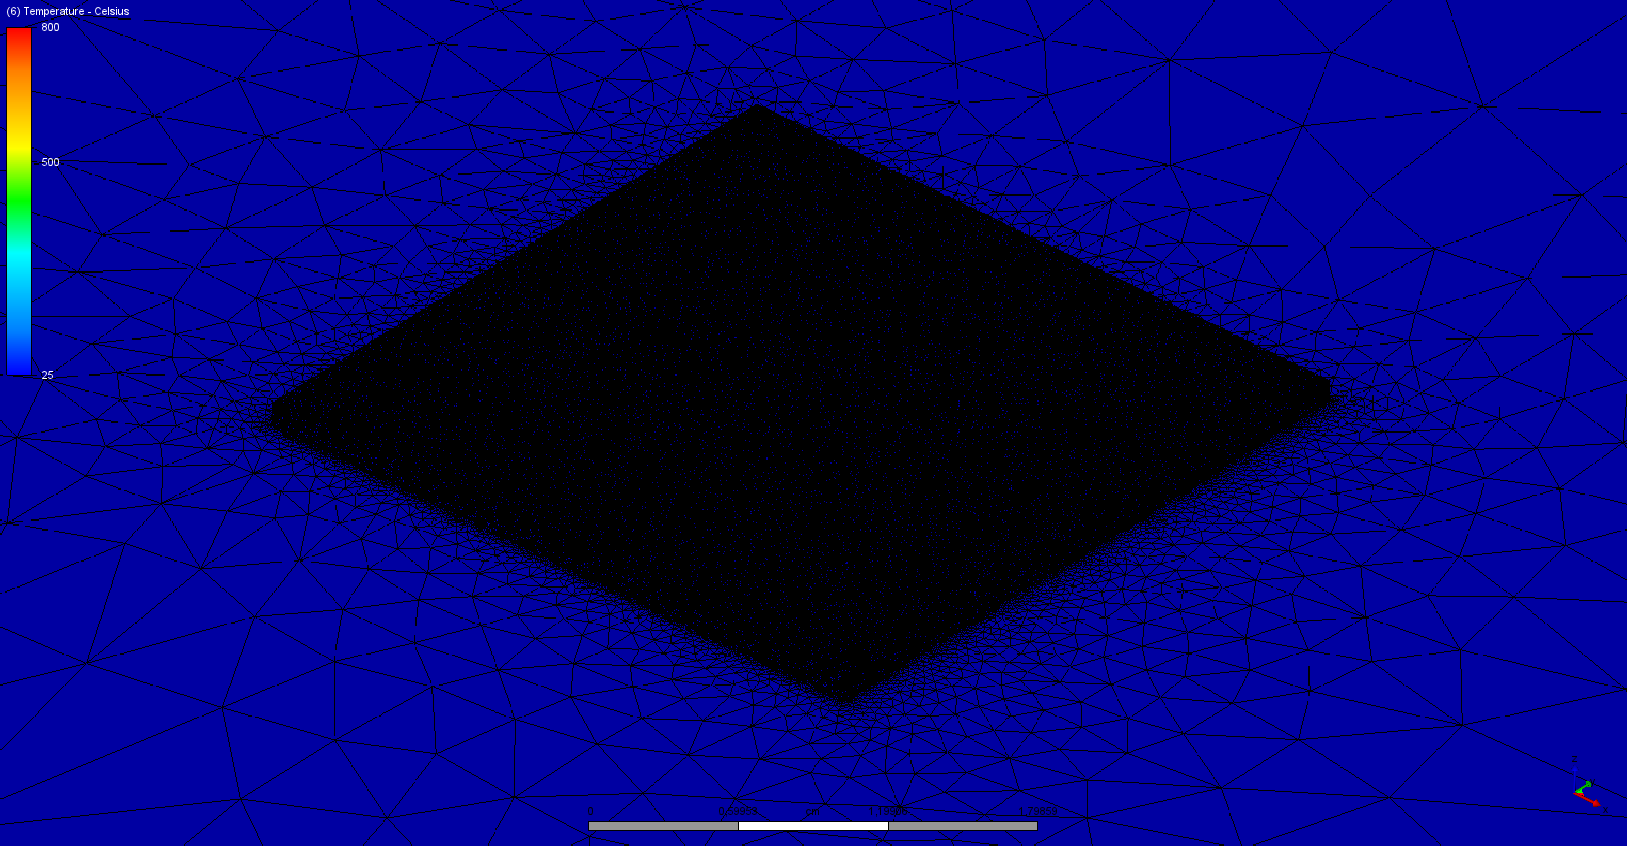
\includegraphics[width=1.00\textwidth]{figuras/Procedimiento_Simulaciones/Conduccion/mallado_100.png}
		\caption{Mallado del nano-espaciador de 100nm}
		\label{fig:mallado_100_metodos}
	\end{subfigure}
	\hfill
	\begin{subfigure}[b]{0.3\textwidth}
		\centering
			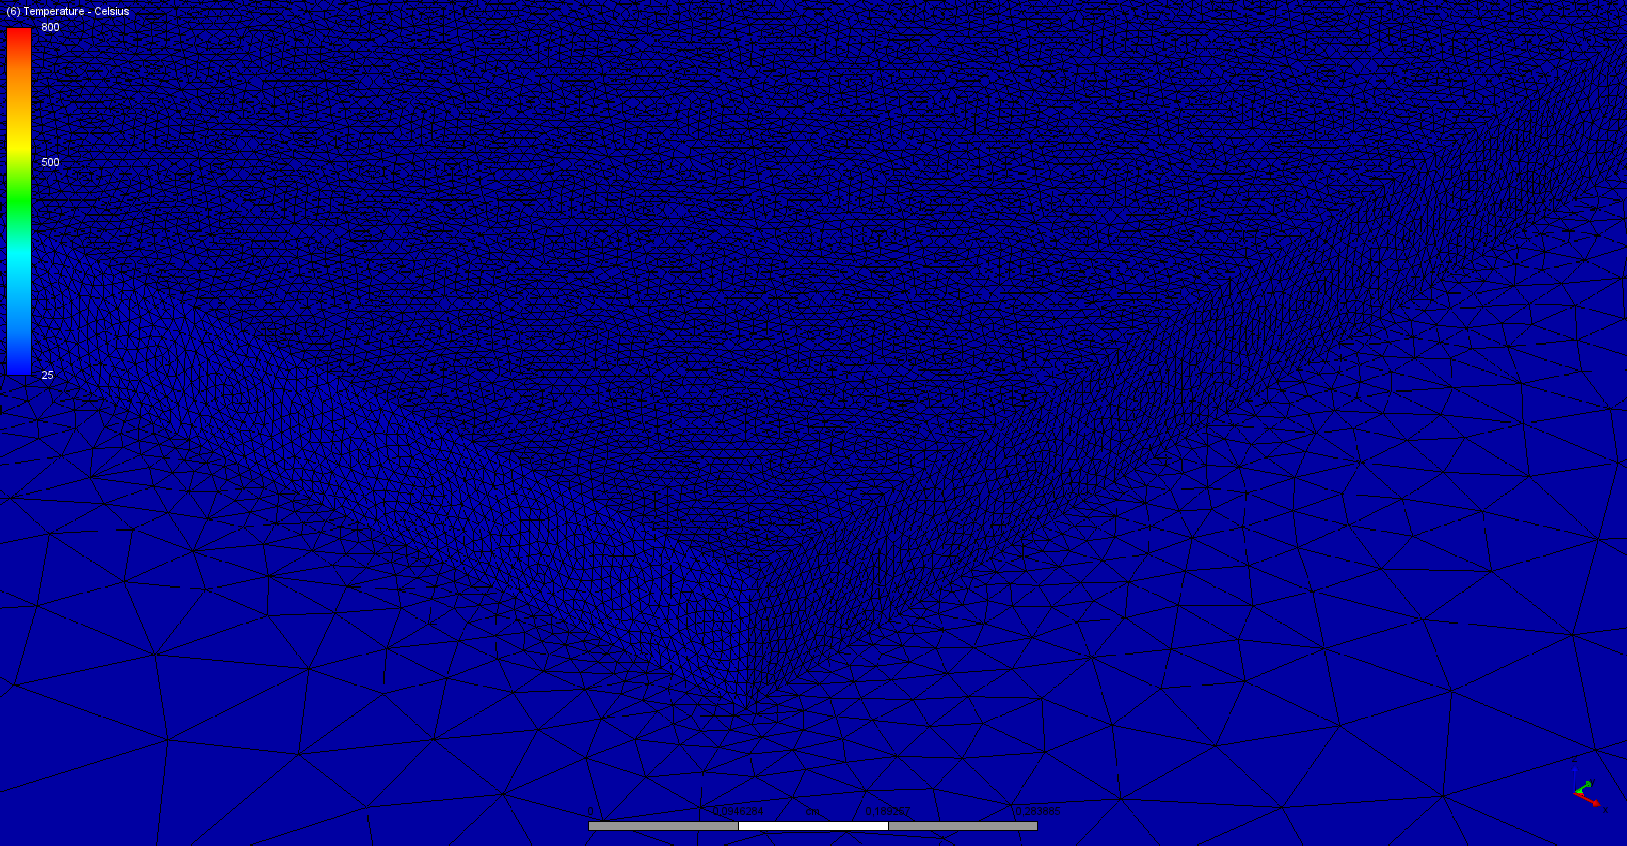
\includegraphics[width=1.00\textwidth]{figuras/Procedimiento_Simulaciones/Conduccion/mallado_100_cerca.png}
		\caption{Mallado del nano-espaciador de 100nm de cerca}
		\label{fig:mallado_100_cerca_metodos}
	\end{subfigure}
	\hfill
	\begin{subfigure}[b]{0.3\textwidth}
		\centering
			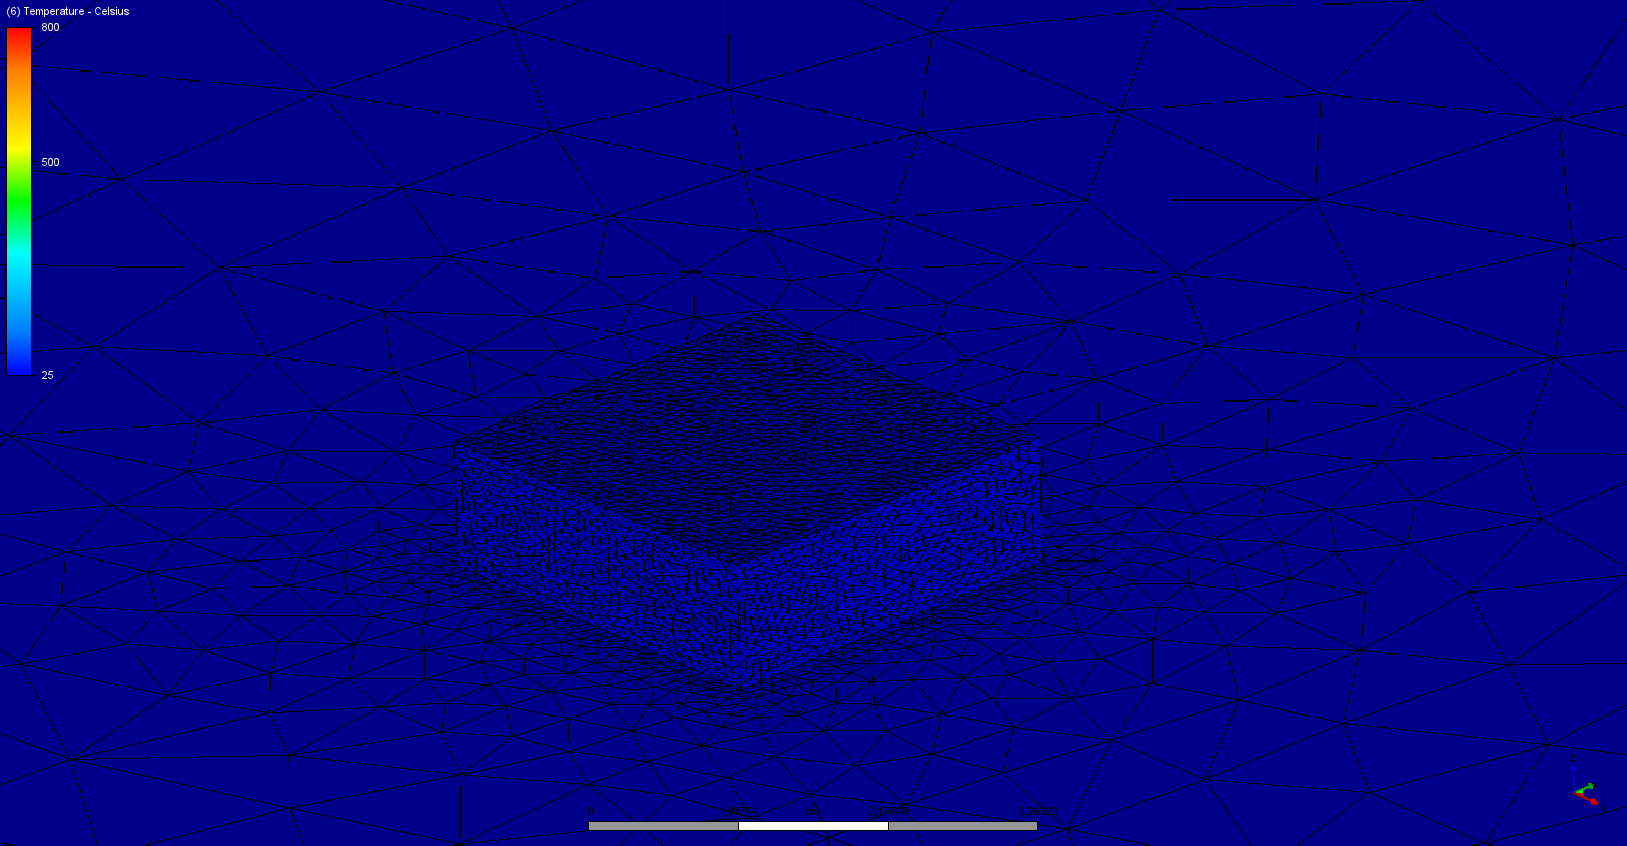
\includegraphics[width=1.00\textwidth]{figuras/Procedimiento_Simulaciones/Conduccion/mallado_1000.png}
		\caption{Mallado del nano-espaciador de 1000nm}
		\label{fig:mallado_1000_cerca_metodos}
	\end{subfigure}
	\caption{(\subref{fig:mallado_100_metodos}) Mallado del nano-espaciador de 100nm, con tamaño de malla de 0.01. (\subref{fig:mallado_100_cerca_metodos}) Mallado del nano-espaciador de 100nm visto de cerca. (\subref{fig:mallado_1000_cerca_metodos}) Mallado del nano-espaciador de 1000nm, con tamaño de malla de 0.1.}
	\label{fig:mallados_metodos}
\end{figure} 
%%% CONTINUA ENUMERACION
	\item Hacer clic en \textbf{Solve} (figura \ref{fig:paneles}).
	\item Seleccionar en la pestaña \textbf{Physics} la casilla de \textbf{Heat transfer} (\ref{fig:physics_panel}) .
	\item Ir a la pestaña \textbf{Control} (figura \ref{fig:control_panel}).
	\item Poner el guardado de los resultados de la simulación a la mitad del número de iteraciones.
	\item Hacer unas 10 a 14 iteraciones asegurándose que continua desde la iteración cero.
	\item Correr la simulación dando click al botón de \textbf{Solve} dentro de la ventana del lanzar la simulación.
	%%% VENTANA DEL SOLVER
	\begin{figure}[h]
		\centering
		\begin{subfigure}[b]{0.48\textwidth}
			\centering
			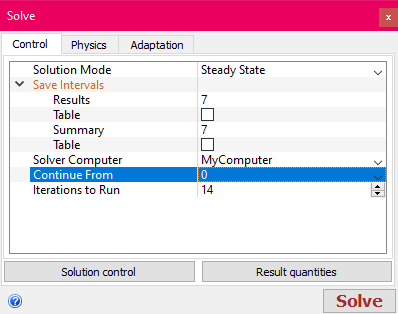
\includegraphics[width=0.8\textwidth]{figuras/Procedimiento_Simulaciones/Conduccion/control_panel.png}
			\caption{panel de control del solver}
			\label{fig:control_panel}
		\end{subfigure}
	  \hfill
		\begin{subfigure}[b]{0.48\textwidth}
			\centering
			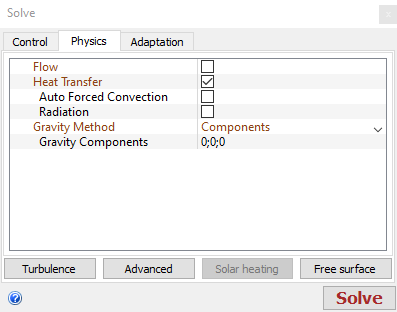
\includegraphics[width=0.8\textwidth]{figuras/Procedimiento_Simulaciones/Conduccion/physics_panel.png}
			\caption{panel de la física del solver}
			\label{fig:physics_panel}
		\end{subfigure}
		\caption{(\subref{fig:control_panel}) Panel de control de la ventana del Solver.(\subref{fig:physics_panel}) Panel de las propiedades físicas de la ventana del Solver.}
		\label{fig:panels_Solver}
	\end{figure}
	%%    CONTINUA
	\item Esperar a que la simulación termine. Un mensaje aparecerá en la ventana de salidas de que la simulación ha finalizado.
	%% Extracción de los resultados
	\item \textbf{Extraer los datos de la simulación en un archivo CSV}.\label{it:extraerResCFD}
	\begin{enumerate}
		\item Abrir la herramienta \textbf{Wall Calculator} con un clic (figura \ref{fig:paneles_resultados}).
		\item Seleccionar las casillas de potencia y temperatura.
		\item Seleccionar la opción de superficie del \textbf{Model entity selection}.
		\item Seleccionar la superficie superior del emisor y la inferior de la célula, aparecerá los números correspondientes a dichas superficies en el \textbf{Wall Calculator} (figura \ref{fig:ventana_wall_calculator_control}).
		\item Hacer clic en \textbf{Calculate}, esto nos llevará a la pestaña de \textbf{Output}.
		\item Hacer clic en \textbf{Write to file} y guardar el archivo de salida que contiene las potencias y temperaturas medias de las superficies seleccionadas (figura \ref{fig:ventana_wall_calculator_resultados}).
	\end{enumerate}
		%%% VENTANA DEL WALL CALCULATOR
	\begin{figure}[h]
		\centering
		\begin{subfigure}[b]{0.48\textwidth}
			\centering
			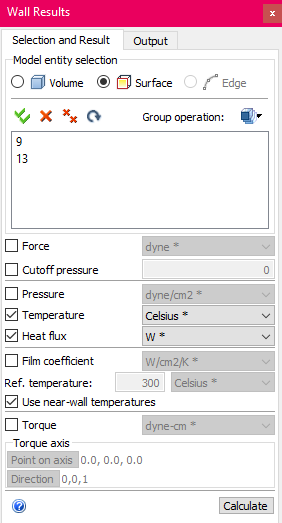
\includegraphics[width=0.6\textwidth]{figuras/Procedimiento_Simulaciones/Conduccion/ventana_wall_calculator.png}
			\caption{Pestaña de selección y resultados.}
			\label{fig:ventana_wall_calculator_control}
		\end{subfigure}
	  \hfill
		\begin{subfigure}[b]{0.48\textwidth}
			\centering
			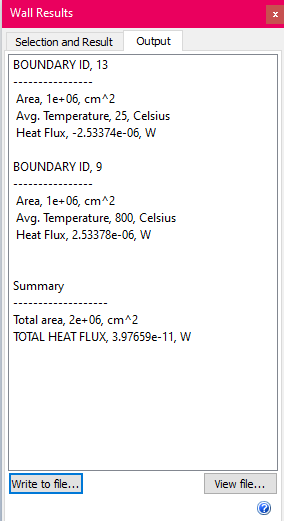
\includegraphics[width=0.6\textwidth]{figuras/Procedimiento_Simulaciones/Conduccion/resultados_conduccion.png}
			\caption{Pestaña de salida.}
			\label{fig:ventana_wall_calculator_resultados}
		\end{subfigure}
		\caption{(\subref{fig:ventana_wall_calculator_control}) Pestaña de selección y resultados del \textbf{Wall Calculator}.(\subref{fig:ventana_wall_calculator_resultados}) Pestaña de salida del \textbf{Wall Calculator}.}
		\label{fig:ventana_wall_calculator}
	\end{figure}
	\item Repetir los pasos anteriores para cada combinación de materiales y resistencias de contacto sin tener que volver a introducir las condiciones de contorno o volver a configurar el mallado.
	\item Repetir los pasos anteriores para cada altura del nano-espaciador.
\end{enumerate}
%%%%%%%%%%%%%%%%%%%%%%%%%%%%%%%%%%%%%%
%            Lista Siglas            %
%%%%%%%%%%%%%%%%%%%%%%%%%%%%%%%%%%%%%% 
\chapter{Lista de siglas}

%\let\cleardoublepage\clearpage
\glsaddall
%\cleardoublepage
%\setglossarysection{chapter}
\setlength{\glsdescwidth}{\textwidth}
\printglossary[type=\acronymtype,title=Acr\'{o}nimos,style=longheader]%superheader]%myacronymstyle]
%\printnoidxglossary[type=\acronymtype,title=Acr\'{o}nimos]%,sort=use]%[type=\acronymtype]
\let\cleardoublepage\clearpage
\chapter{Tabla de Símbolos}
\setlength{\glsdescwidth}{15cm}
\printglossary[type=symbolslist,style=symbunitlong]
\let\cleardoublepage\clearpage
%\printglossary